% ╔══════════════════════════════════════════════════════════════════════════════╗
% ║     PLANTILLA PROFESIONAL - INSTITUTO ATENEO DE COLIMA                     ║
% ║     Investigación Documental: Corrupción en México (2006-2012)               ║
% ║     Diseño: Jerarquía visual + Armonía cromática + Legibilidad              ║
% ╚══════════════════════════════════════════════════════════════════════════════╝

\documentclass[12pt,letterpaper,oneside,openany]{book}

% ═══════════════════════════════════════════════════════════════════════════════
% CONFIGURACIÓN DE MÁRGENES Y GEOMETRÍA (DISEÑO PROFESIONAL)
% ═══════════════════════════════════════════════════════════════════════════════

\usepackage[margin=2.5cm,top=3cm,bottom=3cm,headheight=1.5cm,headsep=0.8cm]{geometry}

% ═══════════════════════════════════════════════════════════════════════════════
% ENCODING, IDIOMA Y TIPOGRAFÍA (DISEÑO PROFESIONAL)
% ═══════════════════════════════════════════════════════════════════════════════

\usepackage[utf8]{inputenc}
\usepackage[T1]{fontenc}
\usepackage[spanish,es-tabla,es-nodecimaldot]{babel}

% Tipografía profesional: Times New Roman para cuerpo, Helvetica para títulos
\usepackage{mathptmx}       % Times New Roman para el cuerpo (serif)
\usepackage{helvet}         % Helvetica para títulos (sans-serif)
\renewcommand{\familydefault}{\rmdefault}  % Cuerpo en serif (Times New Roman)

% ═══════════════════════════════════════════════════════════════════════════════
% PAQUETES ESENCIALES (DISEÑO PROFESIONAL)
% ═══════════════════════════════════════════════════════════════════════════════

\usepackage{graphicx}
\usepackage{xcolor}
\usepackage{colortbl}
\usepackage{booktabs}
\usepackage{longtable}
\usepackage{array}
\usepackage{multirow}
\usepackage{float}
\usepackage{fancyhdr}
\usepackage{titlesec}
\usepackage{setspace}
\usepackage{pdflscape}
\usepackage{amssymb}
\usepackage{amsmath}
\usepackage{url}
\usepackage{eso-pic}                    % Marca de agua mejorada
\usepackage[authoryear,round]{natbib}     % Bibliografía APA
\usepackage[colorlinks=true,linkcolor=ateneo-blue!80!black,citecolor=ateneo-blue!80!black,urlcolor=ateneo-blue!80!black]{hyperref}

% ═══════════════════════════════════════════════════════════════════════════════
% COLORES INSTITUCIONALES - PALETA PROFESIONAL ARMONIZADA
% ═══════════════════════════════════════════════════════════════════════════════

\definecolor{ateneo-primary}{HTML}{A6266C}    % Púrpura institucional (logo)
\definecolor{ateneo-secondary}{HTML}{2E5090}  % Azul académico (títulos)
\definecolor{ateneo-accent}{HTML}{D35400}     % Naranja académico (acento)
\definecolor{ateneo-gray}{HTML}{4A4A4A}      % Gris corporativo (texto)
\definecolor{ateneo-light}{HTML}{F8F9FA}     % Fondo claro (notas)
\definecolor{ateneo-bg}{HTML}{FFFFFF}        % Blanco puro (fondo)

% ═══════════════════════════════════════════════════════════════════════════════
% ESPACIADO Y FORMATO DE PÁRRAFOS (DISEÑO PROFESIONAL)
% ═══════════════════════════════════════════════════════════════════════════════

\setlength{\parindent}{1.25em}  % Sangría profesional
\setlength{\parskip}{0.6em}      % Espacio entre párrafos
\onehalfspacing                   % Interlineado 1.5

% ═══════════════════════════════════════════════════════════════════════════════
% FORMATO DE SECCIONES - JERARQUÍA VISUAL PROFESIONAL
% ═══════════════════════════════════════════════════════════════════════════════

% Capítulo (máxima jerarquía)
\titleformat{\chapter}[display]
  {\normalfont\sffamily\Huge\bfseries\color{ateneo-primary}}
  {\chaptertitlename\ \thechapter}
  {20pt}
  {\Huge}
  [\vspace{5pt}\titlerule\vspace{2pt}\titlerule]

% Sección (jerarquía media)
\titleformat{\section}[block]
  {\normalfont\sffamily\Large\bfseries\color{ateneo-secondary}}
  {\thesection}
  {0.5em}
  {}
  [\vspace{3pt}\titlerule]

% Subsección (jerarquía secundaria)
\titleformat{\subsection}[block]
  {\normalfont\sffamily\large\bfseries\color{ateneo-gray}}
  {\thesubsection}
  {0.5em}
  {}

% Subsubsección (jerarquía terciaria)
\titleformat{\subsubsection}[runin]
  {\normalfont\sffamily\normalsize\bfseries\color{ateneo-gray}}
  {\thesubsubsection}
  {0.5em}
  {}
  [. ]

% ═══════════════════════════════════════════════════════════════════════════════
% ENCABEZADOS Y PIES DE PÁGINA - DISEÑO LIMPIO Y PROFESIONAL
% ═══════════════════════════════════════════════════════════════════════════════

\pagestyle{fancy}
\fancyhf{}
\fancyhead[L]{
\includegraphics[height=0.6cm]{img/image1.png}}  % Logo discreto
\fancyhead[R]{\sffamily\small\color{ateneo-gray}Corrupción 2006--2012}
\fancyfoot[C]{\thepage}
\renewcommand{\headrulewidth}{0.2pt}
\renewcommand{\footrulewidth}{0.2pt}
\renewcommand{\headrule}{\color{ateneo-light!50}}
\renewcommand{\footrule}{\color{ateneo-light!50}}

% Estilo especial para portada
\fancypagestyle{portada}{
  \fancyhf{}
  \renewcommand{\headrulewidth}{0pt}
  \renewcommand{\footrulewidth}{0pt}
}

% ═══════════════════════════════════════════════════════════════════════════════
% MARCA DE AGUA - DISEÑO DISCRETO Y PROFESIONAL
% ═══════════════════════════════════════════════════════════════════════════════

\AddToShipoutPictureBG{%
  \AtPageLowerLeft{%
    \color{ateneo-light!30}% Color muy claro
    \rule{0.2\paperwidth}{\paperheight}% Barra vertical discreta
  }
  \AtPageUpperLeft{%
    \put(50, -50){% Posición discreta
      \color{ateneo-light!50}% Color casi imperceptible
      \scalebox{0.8}{\sffamily\textbf{Estudio Documental}}% Texto pequeño
    }
  }
}

% ═══════════════════════════════════════════════════════════════════════════════
% COMANDOS PERSONALIZADOS - DISEÑO PROFESIONAL
% ═══════════════════════════════════════════════════════════════════════════════

\newcommand{\nota}[1]{%
  \vspace{0.5em}
  \begin{center}
  \fcolorbox{ateneo-secondary!20}{ateneo-light}{\parbox{0.9\textwidth}{\small\textbf{\color{ateneo-secondary}Nota metodológica:} #1}}
  \end{center}
  \vspace{0.5em}
}

\newcommand{\pendiente}[1]{\textcolor{ateneo-accent}{[\textbf{PENDIENTE:} #1]}}

\newcommand{\siglas}[1]{\textsc{\lowercase{#1}}}

\newcommand{\destacar}[1]{\textcolor{ateneo-secondary}{\textbf{#1}}}

% ═══════════════════════════════════════════════════════════════════════════════
% METADATOS DEL DOCUMENTO
% ═══════════════════════════════════════════════════════════════════════════════

\title{%
  {\sffamily\bfseries\color{ateneo-primary}INSTITUTO ATENEO DE COLIMA}\\[0.2cm]
  {\small INCORPORADO A LA UNIVERSIDAD DE COLIMA}\\[1.5cm]
  {\Huge\bfseries\color{ateneo-secondary}Corrupción en México durante el sexenio}\\
  {\Huge\bfseries\color{ateneo-secondary}de Felipe Calderón (2006--2012)}\\[0.5cm]
  {\large Análisis estructural, financiero y de derechos humanos}\\
  {\normalsize a partir de los casos Genaro García Luna, Refinería Bicentenario y Guardería ABC}
}

\author{%
  \textbf{Alumnos:}\\
  Ulysses Emiliano González de la Cruz\\
  Ian Alexander Miramonges Vázquez\\[0.8cm]
  \textbf{Maestra:}\\
  María Elena Luna Angulo\\[0.5cm]
  \textbf{Materia:}\\
  Metodología de la Investigación
}

\date{\today}

% ═══════════════════════════════════════════════════════════════════════════════
% DOCUMENTO PRINCIPAL
% ═══════════════════════════════════════════════════════════════════════════════

\begin{document}

% ───────────────────────────────────────────────────────────────────────────────
% PORTADA INSTITUCIONAL - DISEÑO PROFESIONAL
% ───────────────────────────────────────────────────────────────────────────────

\thispagestyle{portada}
\begin{center}
  \vspace*{1cm}
  
  % Logo institucional
  
\includegraphics[height=2.5cm]{img/image1.png}\\[1.5cm]
  
  {\sffamily\bfseries\color{ateneo-primary}INSTITUTO ATENEO DE COLIMA}\\[0.2cm]
  {\small INCORPORADO A LA UNIVERSIDAD DE COLIMA}\\[2cm]
  
  % Línea decorativa sutil
  {\color{ateneo-light!50}\rule{0.6\textwidth}{0.5pt}}\\[0.5cm]
  
  {\Huge\bfseries\color{ateneo-secondary}Corrupción en México durante el sexenio}\\
  {\Huge\bfseries\color{ateneo-secondary}de Felipe Calderón (2006--2012)}\\[0.8cm]
  
  {\large Análisis estructural, financiero y de derechos humanos}\\
  {\normalsize a partir de los casos Genaro García Luna, Refinería Bicentenario y Guardería ABC}\\[1.5cm]
  
  % Línea decorativa sutil
  {\color{ateneo-light!50}\rule{0.4\textwidth}{0.5pt}}\\[2cm]
  
  % Información académica
  \begin{tabular}{rl}
    \textbf{Materia:} & \sffamily Metodología de la Investigación \\[0.3cm]
    \textbf{Alumnos:} & \sffamily Ulysses Emiliano González de la Cruz \\
                      & \sffamily Ian Alexander Miramonges Vázquez \\[0.3cm]
    \textbf{Maestra:} & \sffamily María Elena Luna Angulo \\[0.3cm]
    \textbf{Fecha:} & \sffamily \today
  \end{tabular}
  
  \vfill
  
  {\footnotesize Colima, México}
  
\end{center}

\clearpage

% ───────────────────────────────────────────────────────────────────────────────
% DECLARACIÓN METODOLÓGICA
% ───────────────────────────────────────────────────────────────────────────────

\thispagestyle{fancy}

\begin{center}
  {\Large\sffamily\bfseries\color{ateneo-secondary}Declaración metodológica}
\end{center}

\vspace{1cm}

\nota{
  Este documento constituye un \textbf{estudio documental} de casos múltiples 
  conforme a los estándares de Hernández Sampieri, Fernández Collado y Baptista 
  Lucio (2014). La investigación se estructuró bajo un \textbf{Diseño Anidado 
  Concurrente de Modelo Dominante (DIAC: CUAL + cuan)} que articula evidencia 
  cualitativa documental triangulada (resoluciones judiciales, auditorías oficiales 
  y doctrina académica) con indicadores cuantitativos secundarios descriptivos 
  (IPC 2025, ENCIG 2025, montos auditados). Los hallazgos ofrecen alcance 
  \textbf{analíticamente transferible} pero no estadísticamente generalizable 
  a la Administración Pública Federal 2006--2012.
}

\vspace{2cm}

\begin{center}
  {\sffamily\bfseries\color{ateneo-secondary}ÍNDICE DE CONTENIDOS}
\end{center}

\tableofcontents

\clearpage

% ═══════════════════════════════════════════════════════════════════════════════
% CONTENIDO PRINCIPAL
% ═══════════════════════════════════════════════════════════════════════════════

\chapter*{Resumen ejecutivo}
\addcontentsline{toc}{chapter}{Resumen ejecutivo}

% ═══════════════════════════════════════════════════════════════════════════════
% INTRODUCCIÓN - INSTITUTO ATENEO DE COLIMA
% Estudio Documental: Corrupción en México (2006-2012)
% ═══════════════════════════════════════════════════════════════════════════════

\nota{
  Este capítulo introduce el problema de investigación desde una perspectiva 
  documental basada en evidencia oficial (ASF, SCJN, CNDH, CIDH, DOJ) y doctrina 
  académica arbitrada (Casar y Cejudo 2024; Merino 2024; Sandoval Ballesteros 2024).
}

\section{Contexto y perspectiva}

Con frecuencia, la historia de la corrupción en México suele narrarse al revés: la atención pública se concentra en el escándalo pasajero, la consigna viral o el enfrentamiento partidista, mientras rara vez se analiza con la cabeza fría el proceso institucional que permitió llegar a ese desenlace y el costo humano que recayó sobre la población. Así como detrás de los resultados visibles existen siempre planes, omisiones o rutinas acumuladas, el propósito de este reporte no consistió en repartir culpas por simpatía política ni en reproducir el ruido mediático, sino en examinar ---mediante evidencia oficial, auditorías y resoluciones judiciales--- qué falló estructuralmente en tres episodios decisivos y de qué manera sus secuelas comprometen lo más valioso para una sociedad: la vida, la salud, la seguridad y el patrimonio colectivo.

Desde la perspectiva científica, la corrupción constituye un fenómeno multidimensional que trasciende el plano estrictamente moral o penal para consolidarse como un problema estructural con repercusiones directas sobre el erario, la calidad de los servicios públicos, la vigencia de los derechos humanos y la legitimidad democrática \citep{inegi2016,monsivais2020,reyesheroles2003}. Su persistencia a través de distintas administraciones revela la consolidación de una corrupción sistémica y estructural, en la que las reglas formales son capturadas por redes de poder lícitas e ilícitas y la impunidad se institucionaliza \citep{casar2024,merino2024,sandoval2024}.

En este estudio se delimitó como periodo nuclear el sexenio de Felipe Calderón Hinojosa (2006--2012), administración que concluyó con una calificación de 34 sobre 100 puntos para México en el Índice de Percepción de la Corrupción (IPC) de Transparencia Internacional (2026). Durante esa etapa se gestaron expedientes de alto impacto cuyas consecuencias jurídicas, financieras y sociales se extendieron hasta noviembre de 2026, según se documentó en informes de la Auditoría Superior de la Federación (\siglas{asf}), sentencias de la Suprema Corte de Justicia de la Nación (\siglas{scjn}), recomendaciones de la Comisión Nacional de los Derechos Humanos (\siglas{cndh}), informes de la Comisión Interamericana de Derechos Humanos (\siglas{cidh}) y procesos penales y civiles sustanciados en tribunales de Estados Unidos \citep{asf2013,asf2015,asf2016,cidh2020,cndh2009,doj2024,scjn2010,scjn2025,uif2025,uif2026}.

La investigación examinó tres casos principales representativos de mecanismos diferenciados: la captura del aparato de seguridad pública y el desvío contractual en el caso de Genaro García Luna; las deficiencias de preinversión y los pasivos transexenales en la Refinería Bicentenario en Tula, Hidalgo; y la subrogación desregulada con conflicto de interés en la Guardería ABC. De manera complementaria, se incorporaron dos casos de contraste contemporáneo (el saqueo hospitalario en Veracruz y la Refinería Olmeca en Dos Bocas) con el fin exclusivo de contrastar el impacto verificable sobre las víctimas frente al sesgo del encuadre mediático (framing). El informe se organizó conforme a los estándares metodológicos de Hernández Sampieri, Fernández Collado y Baptista Lucio (2014), integrando justificación, planteamiento, marco teórico fortalecido con doctrina mexicana, diseño mixto DIAC, análisis de casos, discusión de rigor y limitaciones, conclusiones, referencias y apéndices instrumentales.

\section{Objetivos del estudio}

Este estudio documental se propuso tres objetivos centrales:

\begin{itemize}
  \item Analizar los mecanismos causales y los efectos estructurales ---institucionales, financieros y en materia de derechos humanos--- de la corrupción en México durante el sexenio 2006--2012 mediante un diseño mixto de modelo dominante cualitativo (DIAC: CUAL + cuan).
  
  \item Documentar, mediante evidencia oficial verificable, cómo decisiones administrativas adoptadas hace más de una década continuaron generando pasivos fiscales, litigios y demandas de justicia vigentes en 2026.
  
  \item Contrastar el daño real acreditado en auditorías y resoluciones judiciales con las narrativas mediáticas (framing) que suelen simplificar fenómenos complejos en consignas virales.
\end{itemize}

% FIGURA PENDIENTE
\begin{figure}[H]
\centering
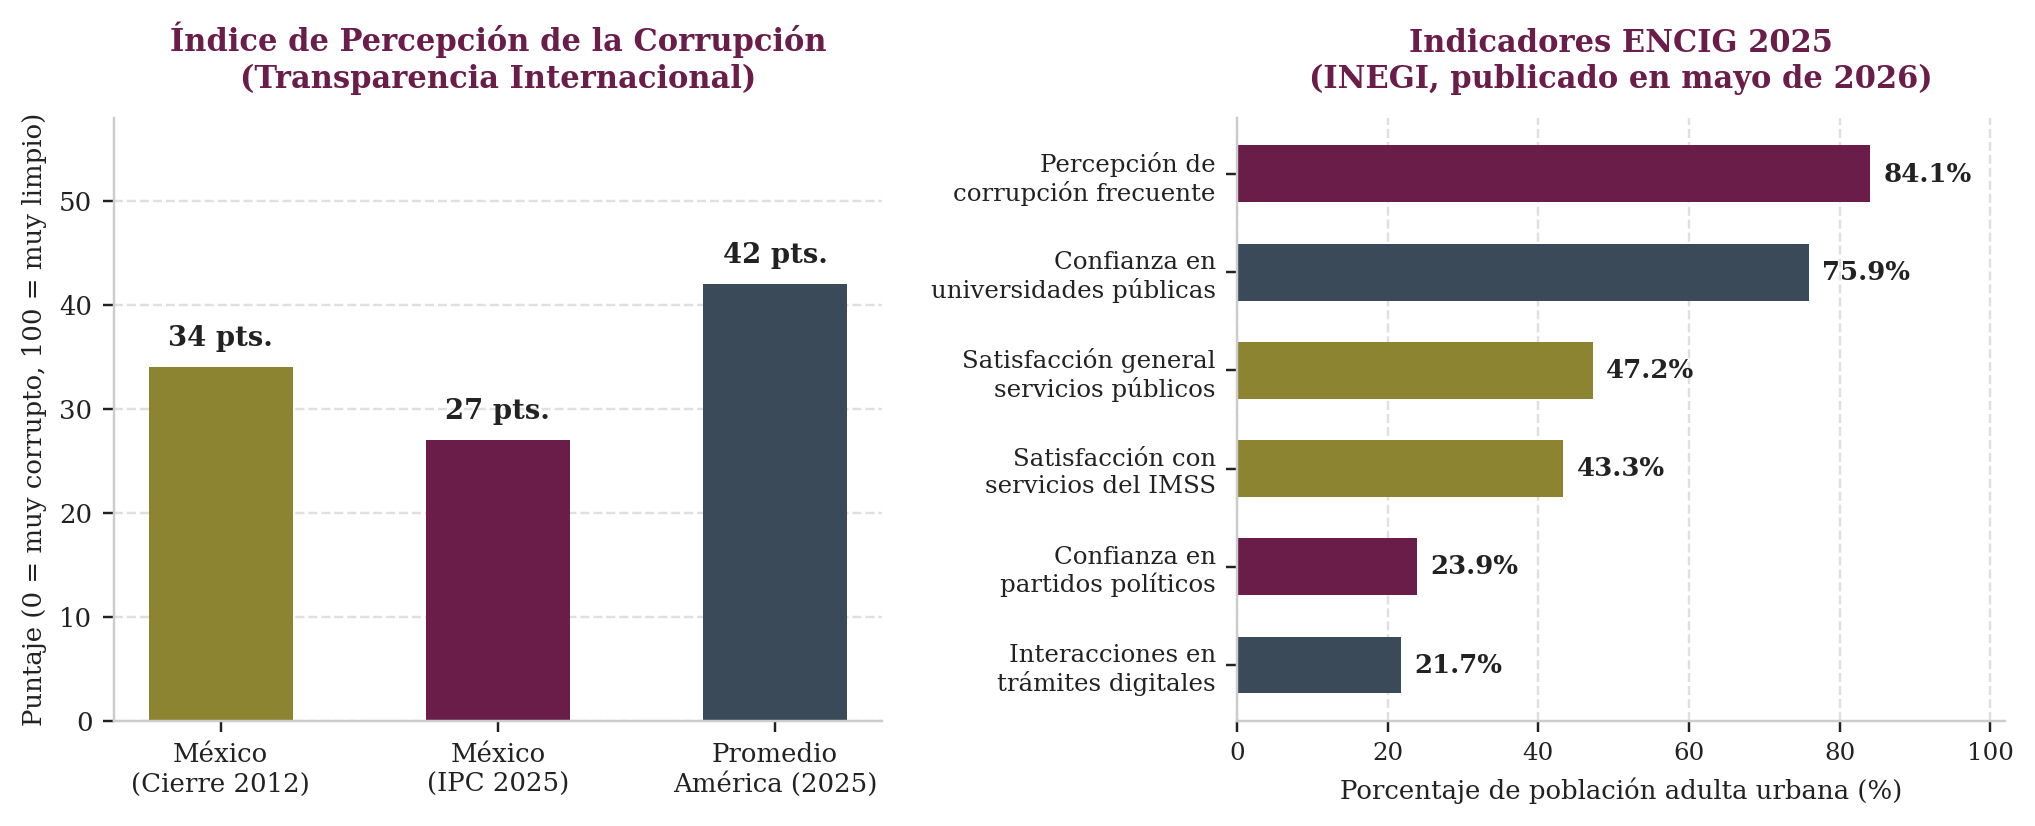
\includegraphics[width=0.9\textwidth]{img/image3.png} % Figura 1: Evolución IPC 2012 vs 2025 + ENCIG 2025
\caption{Evolución del Índice de Percepción de la Corrupción (2012 vs. 2025) e indicadores nacionales de la ENCIG 2025. Fuente: Elaboración propia con datos de Transparencia Internacional (2026) e INEGI (2026).}
\label{fig:ipc-encig}
\end{figure}

\clearpage

\chapter{Introducción}

% ═══════════════════════════════════════════════════════════════════════════════
% INTRODUCCIÓN - INSTITUTO ATENEO DE COLIMA
% Estudio Documental: Corrupción en México (2006-2012)
% ═══════════════════════════════════════════════════════════════════════════════

\nota{
  Este capítulo introduce el problema de investigación desde una perspectiva 
  documental basada en evidencia oficial (ASF, SCJN, CNDH, CIDH, DOJ) y doctrina 
  académica arbitrada (Casar y Cejudo 2024; Merino 2024; Sandoval Ballesteros 2024).
}

\section{Contexto y perspectiva}

Con frecuencia, la historia de la corrupción en México suele narrarse al revés: la atención pública se concentra en el escándalo pasajero, la consigna viral o el enfrentamiento partidista, mientras rara vez se analiza con la cabeza fría el proceso institucional que permitió llegar a ese desenlace y el costo humano que recayó sobre la población. Así como detrás de los resultados visibles existen siempre planes, omisiones o rutinas acumuladas, el propósito de este reporte no consistió en repartir culpas por simpatía política ni en reproducir el ruido mediático, sino en examinar ---mediante evidencia oficial, auditorías y resoluciones judiciales--- qué falló estructuralmente en tres episodios decisivos y de qué manera sus secuelas comprometen lo más valioso para una sociedad: la vida, la salud, la seguridad y el patrimonio colectivo.

Desde la perspectiva científica, la corrupción constituye un fenómeno multidimensional que trasciende el plano estrictamente moral o penal para consolidarse como un problema estructural con repercusiones directas sobre el erario, la calidad de los servicios públicos, la vigencia de los derechos humanos y la legitimidad democrática \citep{inegi2016,monsivais2020,reyesheroles2003}. Su persistencia a través de distintas administraciones revela la consolidación de una corrupción sistémica y estructural, en la que las reglas formales son capturadas por redes de poder lícitas e ilícitas y la impunidad se institucionaliza \citep{casar2024,merino2024,sandoval2024}.

En este estudio se delimitó como periodo nuclear el sexenio de Felipe Calderón Hinojosa (2006--2012), administración que concluyó con una calificación de 34 sobre 100 puntos para México en el Índice de Percepción de la Corrupción (IPC) de Transparencia Internacional (2026). Durante esa etapa se gestaron expedientes de alto impacto cuyas consecuencias jurídicas, financieras y sociales se extendieron hasta noviembre de 2026, según se documentó en informes de la Auditoría Superior de la Federación (\siglas{asf}), sentencias de la Suprema Corte de Justicia de la Nación (\siglas{scjn}), recomendaciones de la Comisión Nacional de los Derechos Humanos (\siglas{cndh}), informes de la Comisión Interamericana de Derechos Humanos (\siglas{cidh}) y procesos penales y civiles sustanciados en tribunales de Estados Unidos \citep{asf2013,asf2015,asf2016,cidh2020,cndh2009,doj2024,scjn2010,scjn2025,uif2025,uif2026}.

La investigación examinó tres casos principales representativos de mecanismos diferenciados: la captura del aparato de seguridad pública y el desvío contractual en el caso de Genaro García Luna; las deficiencias de preinversión y los pasivos transexenales en la Refinería Bicentenario en Tula, Hidalgo; y la subrogación desregulada con conflicto de interés en la Guardería ABC. De manera complementaria, se incorporaron dos casos de contraste contemporáneo (el saqueo hospitalario en Veracruz y la Refinería Olmeca en Dos Bocas) con el fin exclusivo de contrastar el impacto verificable sobre las víctimas frente al sesgo del encuadre mediático (framing). El informe se organizó conforme a los estándares metodológicos de Hernández Sampieri, Fernández Collado y Baptista Lucio (2014), integrando justificación, planteamiento, marco teórico fortalecido con doctrina mexicana, diseño mixto DIAC, análisis de casos, discusión de rigor y limitaciones, conclusiones, referencias y apéndices instrumentales.

\section{Objetivos del estudio}

Este estudio documental se propuso tres objetivos centrales:

\begin{itemize}
  \item Analizar los mecanismos causales y los efectos estructurales ---institucionales, financieros y en materia de derechos humanos--- de la corrupción en México durante el sexenio 2006--2012 mediante un diseño mixto de modelo dominante cualitativo (DIAC: CUAL + cuan).
  
  \item Documentar, mediante evidencia oficial verificable, cómo decisiones administrativas adoptadas hace más de una década continuaron generando pasivos fiscales, litigios y demandas de justicia vigentes en 2026.
  
  \item Contrastar el daño real acreditado en auditorías y resoluciones judiciales con las narrativas mediáticas (framing) que suelen simplificar fenómenos complejos en consignas virales.
\end{itemize}

% FIGURA PENDIENTE
\begin{figure}[H]
\centering
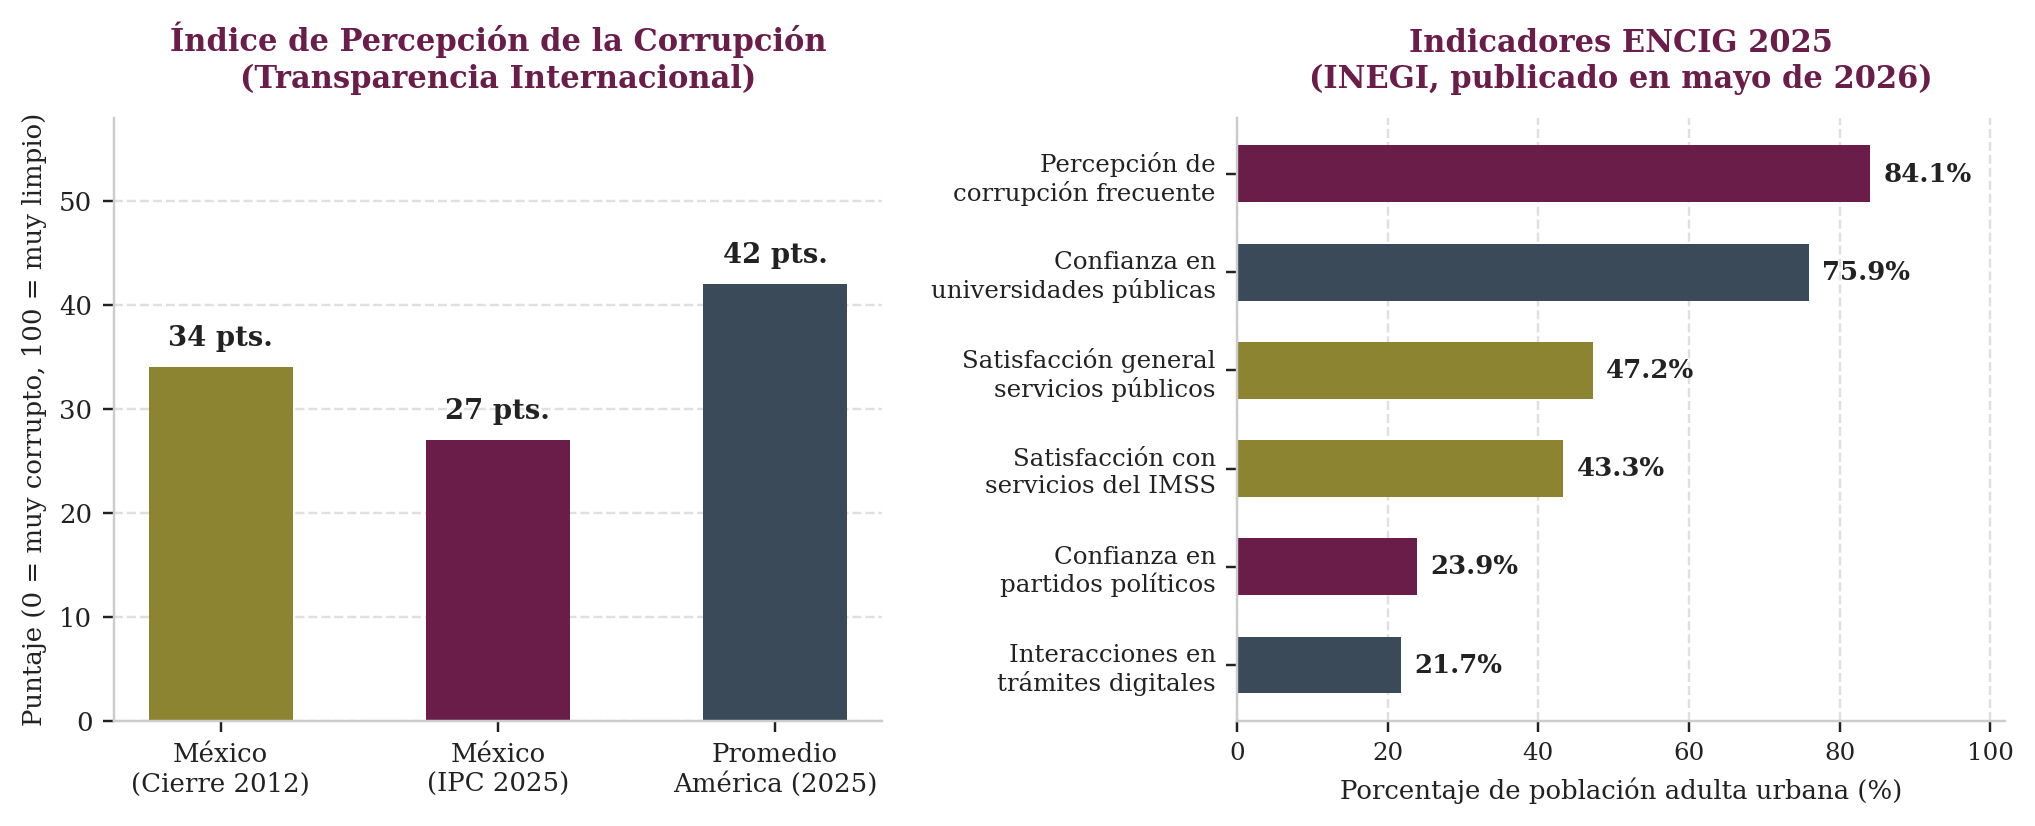
\includegraphics[width=0.9\textwidth]{img/image3.png} % Figura 1: Evolución IPC 2012 vs 2025 + ENCIG 2025
\caption{Evolución del Índice de Percepción de la Corrupción (2012 vs. 2025) e indicadores nacionales de la ENCIG 2025. Fuente: Elaboración propia con datos de Transparencia Internacional (2026) e INEGI (2026).}
\label{fig:ipc-encig}
\end{figure}

\clearpage

\chapter{Justificación de la investigación}

% ═══════════════════════════════════════════════════════════════════════════════
% JUSTIFICACIÓN - INSTITUTO ATENEO DE COLIMA
% Estudio Documental: Corrupción en México (2006-2012)
% ═══════════════════════════════════════════════════════════════════════════════

\nota{
  Esta sección articula cinco dimensiones de justificación metodológica: social, 
  académica, práctica, utilidad metodológica y viabilidad, todas fundamentadas en 
  fuentes oficiales verificables y doctrina académica arbitrada.
}

\section{Relevancia social}

La literatura internacional en derechos humanos establece que la corrupción no es un delito sin víctimas, sino una práctica que vulnera directa o indirectamente derechos económicos, sociales y culturales ---entre ellos la vida, la salud, la seguridad y el acceso equitativo a bienes públicos---, afectando de forma desproporcionada a los sectores vulnerables y profundizando la desigualdad estructural \citep{cidh2019,cndh2019,rios2021}. 

En México, el fenómeno opera como un impuesto regresivo de alcance cotidiano: de acuerdo con la Encuesta Nacional de Calidad e Impacto Gubernamental (ENCIG) 2025 del INEGI, publicada en mayo de 2026, 84.1\,\% de la población adulta urbana percibió que los actos de corrupción gubernamental son frecuentes o muy frecuentes, mientras que los pagos indebidos en trámites extrajeron 17,707.4 millones de pesos anuales ---3,865 pesos promedio por víctima---, el costo real más alto de la última década \citep{inegi2026,imco2026}. El análisis retrospectivo de los expedientes clave del periodo 2006--2012 permitió evidenciar cómo decisiones administrativas adoptadas hace más de una década continuaron generando pasivos fiscales, litigios y demandas de justicia vigentes en 2026.

\section{Relevancia académica}

El estudio científico de la corrupción mexicana demanda articular marcos conceptuales internacionales con la tradición académica nacional en ciencia política, sociología, antropología, economía política y derecho público. En esta investigación se integraron aportes clásicos e internacionales ---Nye (1967), Rose-Ackerman (1999, 2004), Garay Salamanca y Salcedo-Albarán (2012), Cancino y el BID (2020), Dávid-Barrett y Fazekas (2020) y Rezzoagli et al. (2021)--- con obras medulares de investigadores mexicanos como Casar y Cejudo (2024), Merino (2024), López Ayllón y Merino (2009), Peschard (2017), Arellano Gault (2012, 2020), Lomnitz (2000), Zaid (2019), Sandoval Ballesteros (2009, 2024), Serna de la Garza (2010), Vázquez Valencia (2019), Astorga (2007, 2015), Flores Pérez (2009) y Reyes Heroles (2003). Dicha articulación permitió contrastar marcos teóricos complejos con resoluciones judiciales y auditorías oficiales verificables.

\section{Relevancia práctica}

Diversos diagnósticos institucionales coinciden en que el principal obstáculo para contener la corrupción en México no radica en la ausencia de legislación, sino en la brecha de implementación entre la norma jurídica y su cumplimiento efectivo \citep{casar2024,lopezayllon2009,peschard2017}. Al reconstruir los factores que hicieron posibles la concentración discrecional del mando policial, la contratación de megainfraestructura sin candados transexenales y la expansión de guarderías subrogadas sin vigilancia independiente, los hallazgos de este trabajo ofrecieron insumos concretos para el diseño de políticas de fiscalización autónoma, digitalización de trámites y control regulatorio sobre servicios concesionados.

\section{Utilidad metodológica}

Desde el punto de vista metodológico, el estudio aportó un procedimiento replicable para investigar fenómenos de gran corrupción mediante un Diseño Anidado Concurrente de Modelo Dominante (DIAC: CUAL + cuan) aplicado a estudios de casos múltiples \citep{hernandez2014}. En lugar de analizar por separado las resoluciones judiciales, las auditorías financieras o el discurso periodístico, se diseñaron y aplicaron dos instrumentos documentales estructurados ---una Ficha de Registro Jurídico-Institucional y Hemerográfico (Apéndice A) y una Matriz Comparativa de Variables, Dimensiones e Indicadores por Caso (Apéndice B)--- que permitieron triangular evidencia probatoria oficial con estadísticas descriptivas secundarias y análisis de encuadre mediático (framing), generando metainferencias trazables.

\section{Viabilidad del estudio}

La investigación resultó plenamente viable desde las dimensiones documental, técnica, temporal y financiera. Se dispuso de acceso abierto a fuentes primarias oficiales y de alta confiabilidad ---informes de la ASF, engroses y dictámenes de la SCJN, recomendaciones de la CNDH, informes de la CIDH, comunicados de la Unidad de Inteligencia Financiera (UIF), expedientes del Departamento de Justicia de Estados Unidos (DOJ), bases estadísticas del INEGI y reportes de Transparencia Internacional---, complementadas con libros y artículos científicos dictaminados. La selección acotada de tres casos principales y dos de contraste contemporáneo garantizó profundidad analítica sin requerir financiamiento externo ni trabajo de campo en entornos de riesgo.

\clearpage

% ═══════════════════════════════════════════════════════════════════════════════
% REFERENCIAS Y APÉNDICES
% ═══════════════════════════════════════════════════════════════════════════════

\nocite{*}
\bibliographystyle{apalike}
\bibliography{referencias-corrupcion-calderon}

\appendix

\chapter{Ficha de Registro Jurídico-Institucional}
% ═══════════════════════════════════════════════════════════════════════════════
% APÉNDICE A: FICHA DE REGISTRO JURÍDICO-INSTITUCIONAL - INSTITUTO ATENEO DE COLIMA
% Estudio Documental: Corrupción en México (2006-2012)
% ═══════════════════════════════════════════════════════════════════════════════

\nota{
  Este apéndice presenta el instrumento documental utilizado para registrar 
  sistemáticamente la evidencia oficial de cada caso. La ficha garantiza 
  trazabilidad y reproducibilidad del análisis documental.
}

\section{Ficha de Registro Jurídico-Institucional y Hemerográfico}

\begin{table}[H]
\centering
\caption{Formato de Ficha de Registro (Apéndice A)}
\label{tab:ficha_registro}
\small
\begin{tabular}{@{}p{4cm}p{10cm}@{}}
\toprule
\textbf{Campo de registro} & \textbf{Descripción operativa / criterio de llenado} \\
\midrule
Código de ficha y fecha & Ej.: F-01 / Fecha de consulta y última verificación (DD/MM/AAAA). \\
\addlinespace
Caso y clasificación muestral & Nombre del caso $|$ [$\Box$] Caso principal (2006--2012) [$\Box$] Caso de contraste contemporáneo (framing). \\
\addlinespace
Periodo de hechos y seguimiento & Años de origen (ej. 2006--2012) y corte de resoluciones judiciales/fiscales (hasta nov. 2026). \\
\addlinespace
Dependencias y actores & Instituciones federales/estatales, contratistas, operadores privados y autoridades jurisdiccionales. \\
\addlinespace
Tipología de irregularidad & [$\Box$] Cohecho [$\Box$] Peculado [$\Box$] Captura estatal [$\Box$] Conflicto de interés [$\Box$] Mala planeación [$\Box$] Negligencia regulatoria. \\
\addlinespace
Fuentes primarias oficiales & Sentencias judiciales (expediente y corte), auditorías ASF (clave), recomendaciones CNDH/CIDH. \\
\addlinespace
Respaldo académico y verificación & Libros arbitrados, artículos científicos y periodismo de verificación. \\
\addlinespace
Posturas de descargo y continuidad & Declaraciones oficiales de defensa y vínculos del esquema con administraciones previas o posteriores. \\
\addlinespace
Categorías codificadas y trazabilidad & Códigos temáticos asignados, estatus procesal y vínculo entre evidencia CUAL y datos cuan. \\
\bottomrule
\end{tabular}
\end{table}

\section{Ejemplo de Ficha Completada: Caso Genaro García Luna}

\begin{table}[H]
\centering
\caption{Ficha de Registro: Caso Genaro García Luna (F-01)}
\label{tab:ficha_ejemplo}
\small
\begin{tabular}{@{}p{4cm}p{10cm}@{}}
\toprule
\textbf{Campo} & \textbf{Contenido} \\
\midrule
Código y fecha & F-01 / 15/11/2026 \\
\addlinespace
Caso & Genaro García Luna (SSP 2006--2012) \\
\addlinespace
Clasificación & [$\times$] Caso principal (2006--2012) [$\Box$] Contraste \\
\addlinespace
Periodo & 2001--2018 (colusión desde 2001; contratos hasta 2018) \\
\addlinespace
Dependencias & SSP, AFI, CISEN, OADPRS, PGJCDMX \\
\addlinespace
Tipología & [$\times$] Cohecho [$\times$] Peculado [$\times$] Captura estatal [$\Box$] Conflicto de interés [$\Box$] Mala planeación [$\Box$] Negligencia \\
\addlinespace
Fuentes primarias & DOJ 19-CR-576 (2024); UIF (2024, 2025, 2026); ASF (contratos tecnológicos) \\
\addlinespace
Respaldo académico & Astorga (2015); Vázquez Valencia (2019); Flores Pérez (2009) \\
\addlinespace
Posturas descargo & Calderón (Infobae 2024): «Nunca tuve evidencia verificable» \\
\addlinespace
Categorías & Captura institucional; macrocriminalidad; red offshore \\
\bottomrule
\end{tabular}
\end{table}

\chapter{Matriz Comparativa de Variables}
% ═══════════════════════════════════════════════════════════════════════════════
% APÉNDICE B: MATRIZ COMPARATIVA - INSTITUTO ATENEO DE COLIMA
% Estudio Documental: Corrupción en México (2006-2012)
% ═══════════════════════════════════════════════════════════════════════════════

\nota{
  Este apéndice presenta la matriz comparativa utilizada para integrar 
  evidencia cualitativa (mecanismos institucionales) con indicadores 
  cuantitativos anidados (montos, víctimas, sentencias). La matriz 
  permite generar metainferencias trazables por caso.
}

\section{Matriz Comparativa de Variables, Dimensiones e Indicadores por Caso}

\begin{landscape}
\begin{table}[H]
\centering
\caption{Matriz Comparativa por Caso (Apéndice B)}
\label{tab:matriz_comparativa}
\tiny
\begin{tabular}{@{}p{2cm}p{2.5cm}p{3.5cm}p{4cm}p{6.5cm}@{}}
\toprule
\textbf{Caso y tipo} & \textbf{Dimensión analítica / factor asociado} & \textbf{Mecanismo institucional (CUAL)} & \textbf{Indicadores cuantitativos (cuan)} & \textbf{Fuentes trianguladas (APA 7)} \\
\midrule
Caso 1 (Principal) \newline Genaro García Luna & Concentración de mando, presupuesto e inteligencia en SSP sin contrapesos. & Captura estatal y macrocriminalidad: cohecho con Cártel de Sinaloa + red offshore Weinberg. & PF: 5,000 a >35,000; 30 contratos (>727 MDD y 528 mdp); prisión >38 años (2024); civiles \textasciitilde2,500 MDD (2025) y >578 MDD (2026). & DOJ (2024, exp. 19-CR-576); UIF (2024, 2025, 2026); Astorga (2015); Vázquez Valencia (2019); Infobae (2024). \\
\addlinespace
Caso 2 (Principal) \newline Refinería Bicentenario & Anuncio político prematuro, preinversión débil y sin candados transexenales. & Opacidad y mala planeación en megainfraestructura con transferencia de pasivos. & Proyección >9,000 MDD; gasto Pemex >9,000 mdp; barda >500 mdp; deuda Hidalgo \textasciitilde1,500 mdp liquidada sep. 2025; 195.5 mdp en 2020. & ASF (2015, 2016); Cancino (2020); Sandoval Ballesteros (2024); El Financiero (2025). \\
\addlinespace
Caso 3 (Principal) \newline Guardería ABC & Desregulación de estancias IMSS, conflicto de interés y omisión de inspecciones. & Subrogación desregulada con dilución de la responsabilidad administrativa estatal. & Subrogadas: 757 a 1,374 (+81.5\,\%) vs. 142 directas; 14 de 40 empleados; 49 fallecidos y >100 lesionados graves. & CNDH (2009); SCJN (2009, 2010, 2025); Núñez Esquer (2026); CIDH (2020); Serna de la Garza (2010); Osorno (2010). \\
\addlinespace
Contraste 1 \newline Sector Salud Veracruz & Saqueo presupuestal y empresas fantasma; encuadre viral impreciso. & Contraste entre rumor mediático («agua destilada») y desvío hospitalario acreditado. & 0 evidencia agua destilada (COFEPRIS); 46,984 pruebas VIH y 16.8 t fármacos caducos; 2,933 mdp obra; >3,617 mdp fantasma. & Secretaría de Salud / COFEPRIS (2017); Connectas (s.\,f.); Animal Político (s.\,f.); Santiago y Morales (2025); Ángel (2025); Sola-Morales y Zurbano-Berenguer (2019). \\
\addlinespace
Contraste 2 \newline Refinería Olmeca / Dos Bocas & Sobrecostos en megainfraestructura y polarización en eslóganes partidistas. & Contraste entre consigna viral («no refina») y desempeño técnico-financiero real. & Costo: 8,000 a >21,000 MDD (\textasciitilde2.6x); producción 212--263 mil bd (fin 2025) con caída a 141 mil bd (jun. 2026). & Alegría (2026); Martínez Escamilla (2026); El Universal / Celaya (2026); Cancino (2020); Reyes Heroles (2003). \\
\bottomrule
\end{tabular}
\end{table}
\end{landscape}

\end{document}